\documentclass[default]{beamer}
\setbeamertemplate{navigation symbols}{}

\usetheme{Frankfurt}
%\useoutertheme{infolines}
\usecolortheme{beaver}

\usepackage[utf8]{inputenc}					% Выбор языка и кодировки
\usepackage[english, russian]{babel}	% Языки: русский, английский
\usepackage{csquotes}

\usepackage{tikz}
\usetikzlibrary{arrows,shapes,calc}
\everymath{\displaystyle}
\tikzstyle{every picture}+=[remember picture]

\usepackage{animate}
\usepackage{fp}
\usepackage{textpos}
\usepackage{multimedia}
\usepackage{media9}
\usepackage{listings}
\usepackage{minted}

\graphicspath{{../../images/}} 			% Пути к изображениям

\makeatletter
\setbeamertemplate{footline}
{
	\leavevmode%
	\hbox{%
		\begin{beamercolorbox}[wd=.333333\paperwidth,ht=2.25ex,dp=1ex,center]{author
				in head/foot}%
			\usebeamerfont{author in
				head/foot}\insertshortauthor~~\beamer@ifempty{\insertshortinstitute}{}{(\insertshortinstitute)}
		\end{beamercolorbox}%
		\begin{beamercolorbox}[wd=.333333\paperwidth,ht=2.25ex,dp=1ex,center]{title in
				head/foot}%
			\usebeamerfont{title in head/foot}\insertshorttitle
		\end{beamercolorbox}%
		\begin{beamercolorbox}[wd=.333333\paperwidth,ht=2.25ex,dp=1ex,right]{date in
				head/foot}%
			\usebeamerfont{date in head/foot}\insertshortdate{}\hspace*{2em}
			\insertframenumber{}\hspace*{2ex} 
		\end{beamercolorbox}
	}%
	\vskip0pt%
}


\begin{document}
	
	\title[РобоНИС]{НИС: методы искусственного интеллекта в робототехнике}
	\author[Панов, Яковлев]{\textbf{Александр Панов и Константин Яковлев}}
	\institute[ВШЭ]{НИУ ВШЭ}
	\date{16 октября 2017} 
	
	{
	\setbeamertemplate{headline}{}
	\begin{frame}
		
		\titlepage
		\centering
		\href{mailto:apanov@hse.ru}{apanov@hse.ru}
		
		
\includegraphics[width=25pt]{misc/logos/hse.png} \hspace{10pt}
		
\includegraphics[width=100pt]{misc/logos/ras.png} \hspace{10pt}
		
\includegraphics[width=80pt]{misc/logos/frccsc.png}
		
	\end{frame}
	}	

	\section{Обучение с подкреплением}
	\subsection{1}
	\begin{frame}
		\frametitle{Техническое}
		
		\centering
		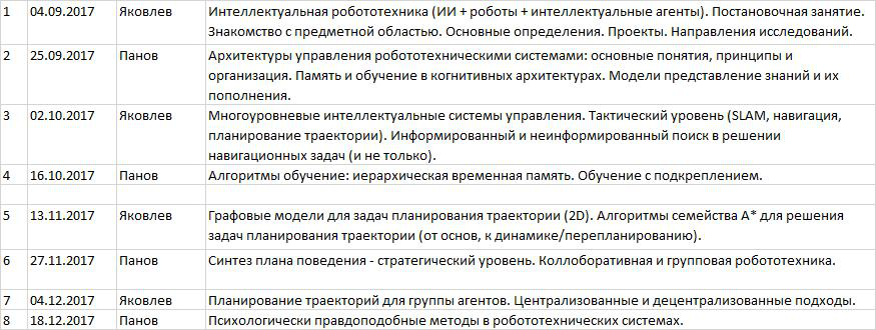
\includegraphics[width=0.9\textwidth]{misc/robots/schedule.png}
		
		\par\bigskip
		
		Обсуждение, вопросы, презентации и ДЗ - на странице курса на Piazza piazza.com/hse.ru/fall2017/aicognitive004
		
	\end{frame}


	\begin{frame}
		\frametitle{Обучение с подкреплением: постановка задачи}
		
		\begin{columns}
			\begin{column}{0.6\textwidth}
				\centering
				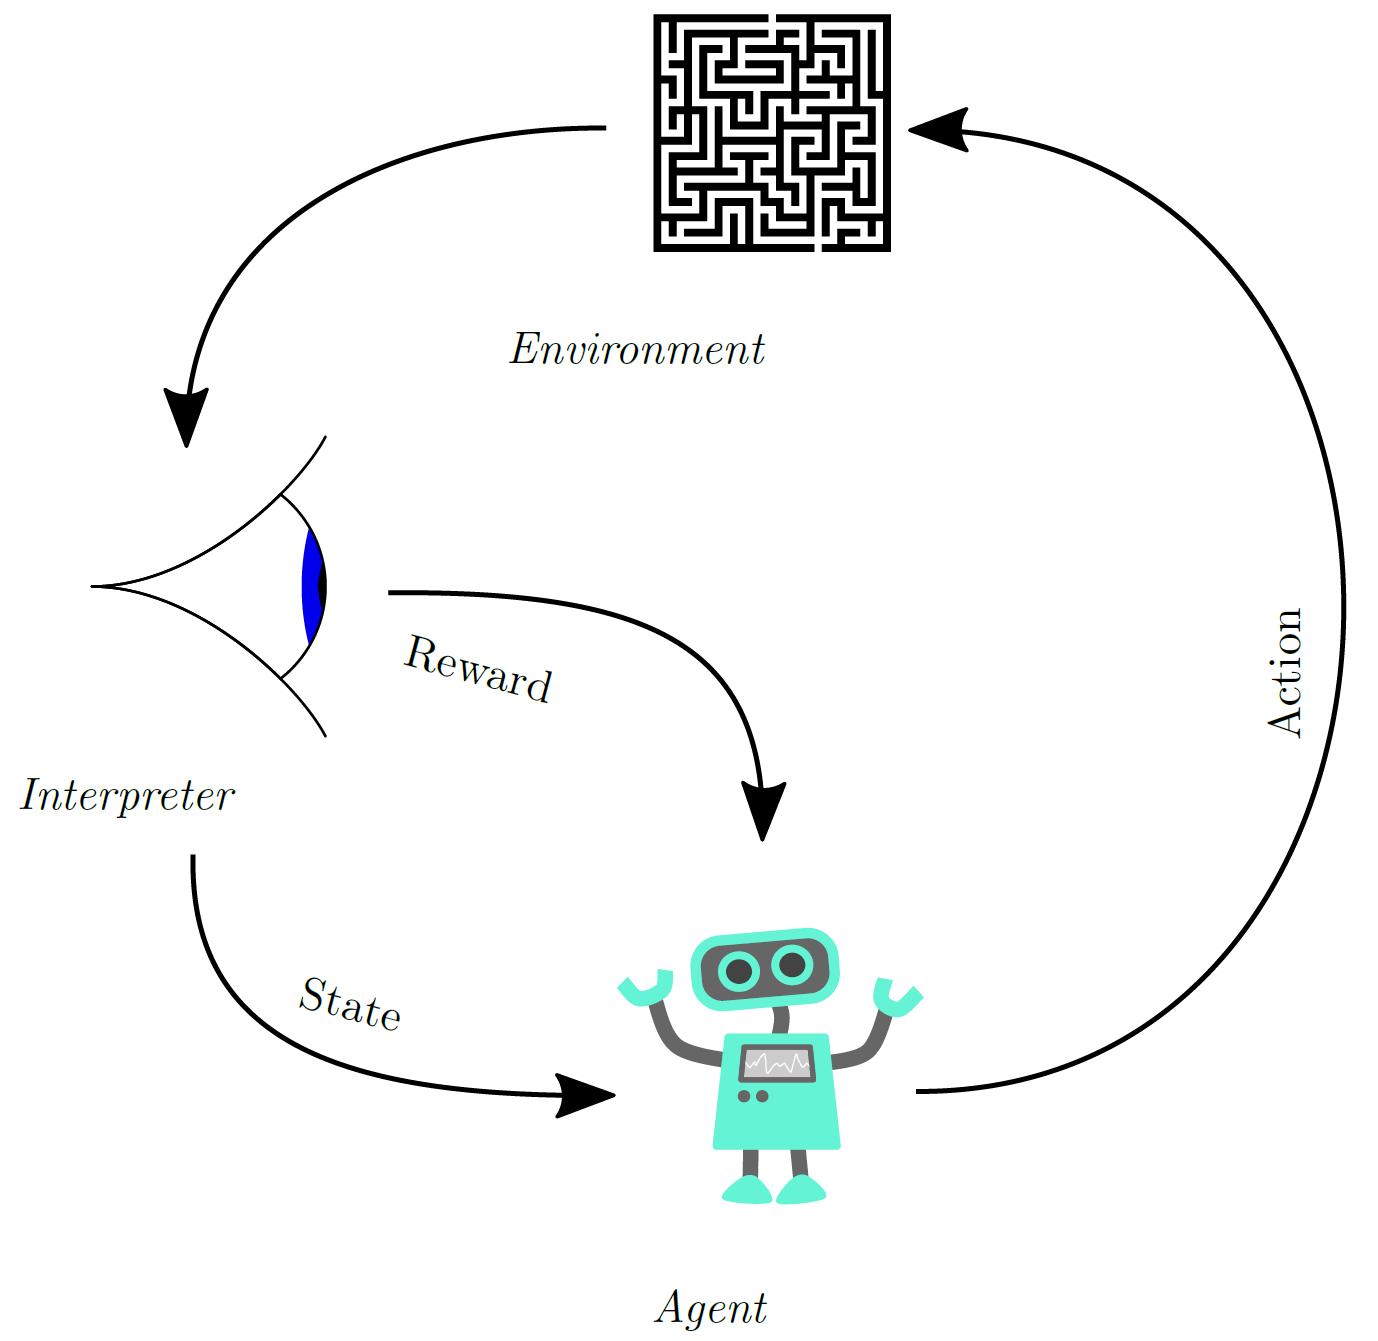
\includegraphics[width=0.8\textwidth]{rl_simple.png}
				
				\par\bigskip
				
				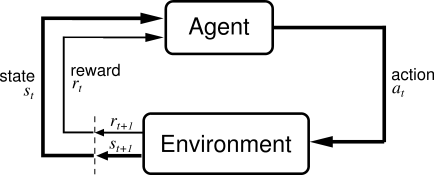
\includegraphics[width=0.8\textwidth]{rl_intro.png}
			\end{column}
			\begin{column}{0.5\textwidth}
				\begin{itemize}
					\item $t$ - дискретные моменты времени,
					\item $a_t\in A$ - действие агента в момент времени $t$,
					\item $E$ - среда, $s_t\rightarrow s_{t+1}$ - состояния среды,
					\item $r_t$ - вознаграждение, поступающее от среды,
					\item $R=\sum\limits_{t}{{{\gamma }^{t}}}{{r}_{t}}$ - суммарное вознаграждение, $0<\gamma \le 1$  - дисконтирующий множитель.
				\end{itemize}
			\end{column}

		\end{columns}
		
	\end{frame}	

	\begin{frame}
		\frametitle{Марковский процесс}
		
		\begin{center}
			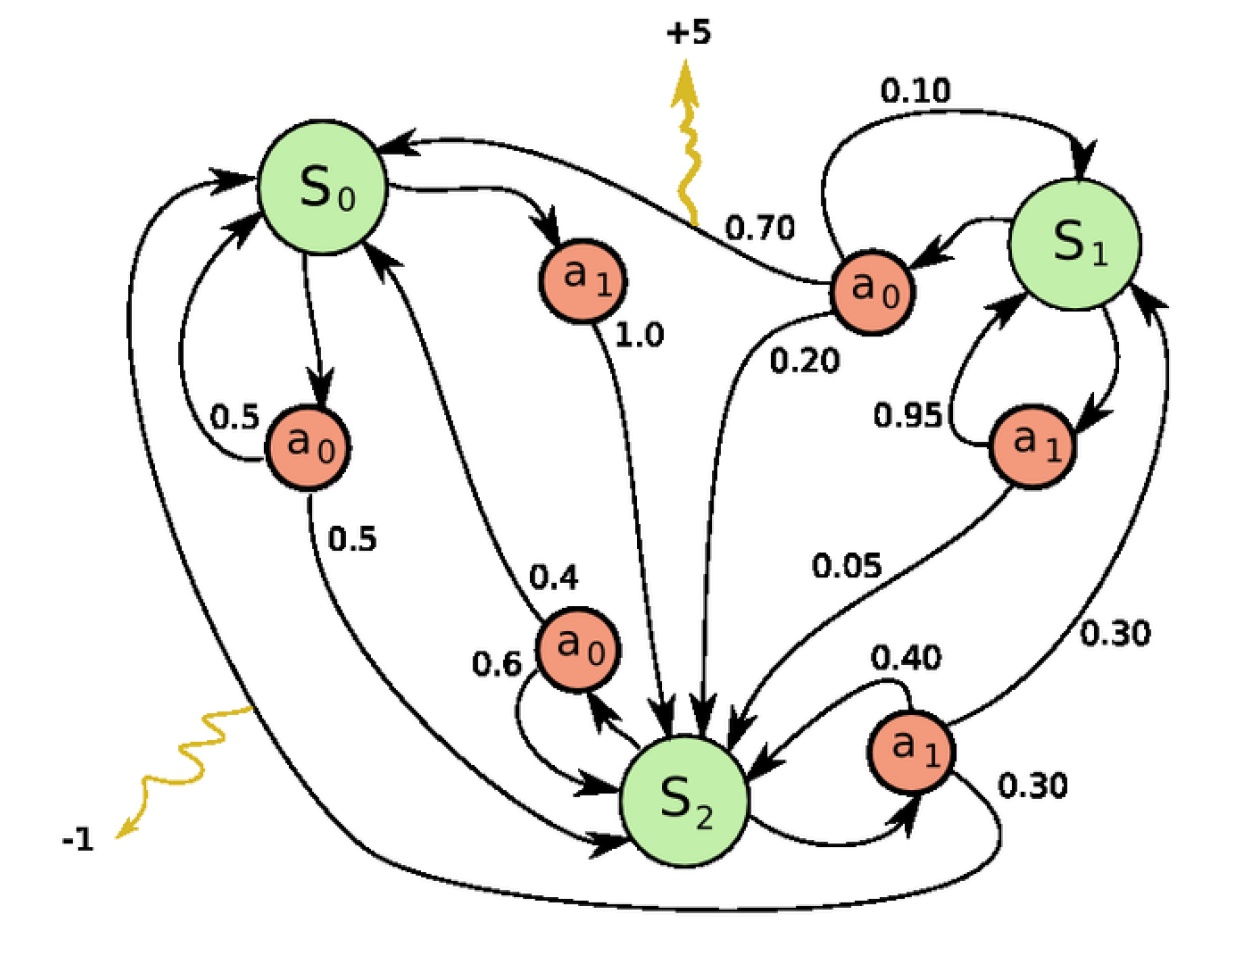
\includegraphics[width=0.4\textwidth]{mdp.png}
		\end{center}
		\par\bigskip
		
		Марковский процесс (Markov decision process (MDP)) - кортеж $\langle S, A, P, R\rangle$:
		\begin{itemize}
			\item $S$ - конечное число состояний,
			\item $A$ - конечное число действий
			\item $P=\{P_a(s,s')=P(s_{t+1}=s'|s_t=s, a_t=a)\}$ - вероятности переходов,
			\item $R=\{r_a(s,s')\}$ - вознаграждение.
		\end{itemize}
		
		
	\end{frame}

	\begin{frame}
		\frametitle{Стратегия агента}

			Цель агента - обучиться стратегии $\pi$ выбора действия в наблюдаемых состояниях среды $\pi:S\to A$, в результате применения которой он получит максимальное суммарное вознаграждение $R$:
			
			\[
				\sum\limits_t\gamma^t r_t \rightarrow \max_\pi
			\] 
			\par\bigskip
			
			Баланс между исследованием среды и учетом предыдущего опыта (exploration vs explotation) - $\varepsilon$-жадный метод:
			\begin{itemize}
				\item с вероятность $1-\varepsilon$ выбирается действие на основе предыдущих прецедентов,
				\item с вероятностью $\varepsilon$- случайное действие из доступных на данный момент
			\end{itemize}
			Параметр $\varepsilon$ уменьшают с течением времени.
	\end{frame}

	\begin{frame}
		\frametitle{Способы решения}

		\begin{itemize}
			\item Если известны $P(s_t,a_t,s_{t+1})$ и $R(s_t,a_t)$, то это задача, основанная на модели, решение \textit{уравнения Беллмана}:
			\[
				V(s)=\max_a Q(s,a),
			\]
			\[
				Q(s,a)=\sum_{s_{t+1}} P(s_t,a_t,s_{t+1})\left(R(s_t,a_t) + \gamma V(s_{t+1})\right),
			\]
			
			где $V(s)=\mathbf{E}[R|s,\pi]$ - функция полезности, а $Q(s,a)=\mathbf{E}[R|s,a,\pi]$ -  функция полезности действия.

			\item Оценка функций полезности $V(s)$ или $Q(s,a)$.
		\end{itemize}
		
		
	\end{frame}

	\begin{frame}

		\frametitle{Обучение с подкреплением: правила перемещения}
		\begin{columns}
			\begin{column}{0.7\textwidth}
				\begin{itemize}
					\item $E=(M,G)$ - среда, где $M$ - карта местности, $G(p_s,p_f)$ - алгоритм генерации вознаграждения,
					\item $a_t=p_t\rightarrow p_{t+1}$ - действия агента по перемещению,
					\item $s_t\in R^{(2d)^2}$ - наблюдения агента (сенсорная информация).
				\end{itemize}
			\end{column}
			\begin{column}{0.3\textwidth}
				\centering
				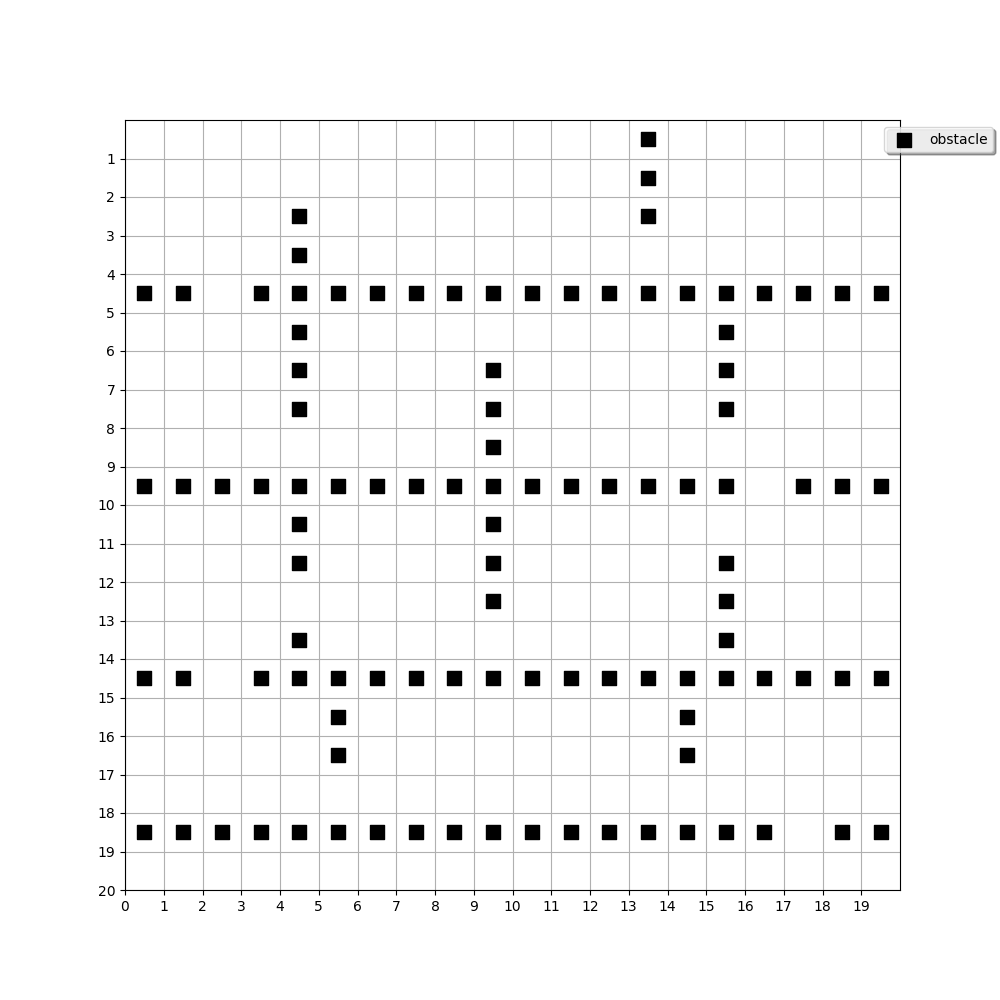
\includegraphics[width=\textwidth]{examples/path/map1}
			\end{column}
		\end{columns}
		\vspace*{10pt}
		Пусть ${{Q}^{*}}({{s}_{t}},{{a}_{t}})={{\max }_{\pi }}\mathbf{E}[R|{{s}_{t}},{{a}_{t}},\pi ]$ - оптимальная функция полезности, тогда с учетом определения $R$ \tikz[baseline] \node[coordinate] (n1) {}; получаем следующее уравнение Беллмана:
		\begin{equation*}
		Q^*(s,a)=\mathbf E_{s_t\sim E}\left[
		\tikz[baseline]{
			\node[fill=blue!20,anchor=base] (t1)
			{$r_t+\gamma\max_{a_t}Q^*(s_t,a_t)$};
		}
		|s,a \right]
		\end{equation*}
		\begin{tikzpicture}[overlay]
		\path[->] (n1.south) edge [bend left, out = 50] (t1);
		\end{tikzpicture}
	\end{frame}
	
	\begin{frame}
		\frametitle{Обучение с подкреплением: аппроксимация}
		
		Для решения итерационными методами уравнения Беллмана используют различные аппроксимации функции ${{Q}^{*}}(s,a)$: $Q(s,a;\theta )\approx {{Q}^{*}}(s,a)$. 
		\par\medskip
		В процессе обучения происходит настройка параметров $\theta$ в результате минимизации функции потерь $L(\theta)$:
		
		\begin{multline*}
		L_i(\theta_i)=\mathbf E_{s,a\sim\rho(\cdot)}\left[(
		\tikz[baseline]{
			\node[fill=blue!20,anchor=base] (t1)	
			{$y_i$};
		}
		-Q(s,a;\theta_i))^2\right],\\
		y_i=
		\tikz[baseline]{
			\node[fill=green!20,anchor=base] (t2)
			{$\mathbf E_{s_t\sim E}\left[r_t+\gamma\max_{a_t}Q(s_t,a_t;\theta _{i-1})|s,a \right]$};
		}
		\end{multline*}
		
		\begin{multline*}
		{{\nabla }_{{{\theta }_{i}}}}{{L}_{i}}({{\theta }_{i}})={{\mathbf{E}}_{s,a\sim \rho (\cdot );{{s}_{t}}\sim E}}\left[ \left( {{r}_{t}}+\gamma {{\max }_{{{a}_{t}}}}Q({{s}_{t}},{{a}_{t}};{{\theta }_{i-1}}) \right. \right.- \\ 
		\left. \left. -Q(s,a;{{\theta }_{i}}) \right){{\nabla }_{{{\theta }_{i}}}}Q(s,a;{{\theta }_{i}}) \right].
		\end{multline*}
		
		
		\begin{tikzpicture}[overlay]
		\path[<-] (t1.north) edge [bend left,in = 120] (t2);
		\end{tikzpicture}
	\end{frame}

	\begin{frame}
		\frametitle{Обучение с подкреплением: переигровки}
		\begin{itemize}
			\item Эпизод - это набор действий агента и реакций среды на перемещения от начального положения до конечно, либо до достижения максимального количества действий $N_a$,
			\item $e_t=(s_t,a_t,r_t,s_{t+1})$ - прецедент сохраняется в память агента $D$,
			\item обучение идет по некоторой случайной выборке $e$ \tikz[baseline] \node[coordinate] (n1) {}; из памяти 
		\end{itemize}
		
		\begin{equation*}
		D=\left\{ e_1, 
		\tikz[baseline]{
			\node[fill=blue!20,anchor=base] (t1)
			{$e_2$};
		}
		,\dots, 
		\tikz[baseline]{
			\node[fill=blue!20,anchor=base] (t2)
			{$e_i$};
		}
		,e_{i+1},\dots e_j,
		\tikz[baseline]{
			\node[fill=blue!20,anchor=base] (t3) 
			{$e_{j+1}$};
		}
		,\dots \right\}
		\end{equation*}
		\begin{tikzpicture}[overlay]
		\path[->] (t1) edge [bend left, out = 50, in=-150] ([xshift=-10pt,yshift=-2pt]n1);
		\path[->] (t2) edge [bend left, out = 40, in=-130] ([xshift=-6pt,yshift=-2pt]n1);
		\path[->] (t3) edge [bend left, out = 30, in=-90] ([xshift=-2pt,yshift=-2pt]n1);
		\end{tikzpicture}
		\begin{itemize}
			\item одно действие можно использовать несколько раз $\rightarrow$ расширяем выборку, устраняем корреляции соседних состояний.
		\end{itemize}
	\end{frame}
		
	\begin{frame}
		\frametitle{Генерация вознаграждения}
		
		Для расчета функции вознаграждения использовали следующий алгоритм:
		\begin{equation*}
		G(s,g,t)=\begin{cases}
		\alpha_{opt}r_t^{opt}+\alpha_{rat}r_t^{rat}+\alpha_{euq}r_t^{euq}, & p_t\leftarrow 0,\\
		r^{obs}, & p_t\leftarrow 1,\\
		r^{tar}, & p_t=g,
		\end{cases}
		\end{equation*}
		где 
		\begin{itemize}
		\item $\sum\alpha_i=1$ - нормировка,
		\item $r_t^{opt}=l_t-l_{t-1}$ - изменение оптимального расстояния,
		\item $r_t^{rat}=e^{-l_t/l_0}$ - штраф за отклонение от цели,
		\item $r_t^{euq}=|p_t-g|-|p_{t-1}-g|$ - регуляризатор для спрямления пути.
		\end{itemize}
	\end{frame}	


	\section{Иерархическая временная память}
	\subsection{2}

	\begin{frame}
		\frametitle{Нейросетевые архитектуры для аппроксимации Q}
		Можно использовать разные варианты сетей:
		\begin{enumerate}
			\item $Ag_1$ - <<мелкая>> полносвязная нейронная сеть,
			\item $Ag_2$ - сверточная сеть средней глубины с полносвязными выходным слоем,
			\item $Ag_3$ - глубокая сеть, состоящая из блоков Inception.
		\end{enumerate}
		\centering
		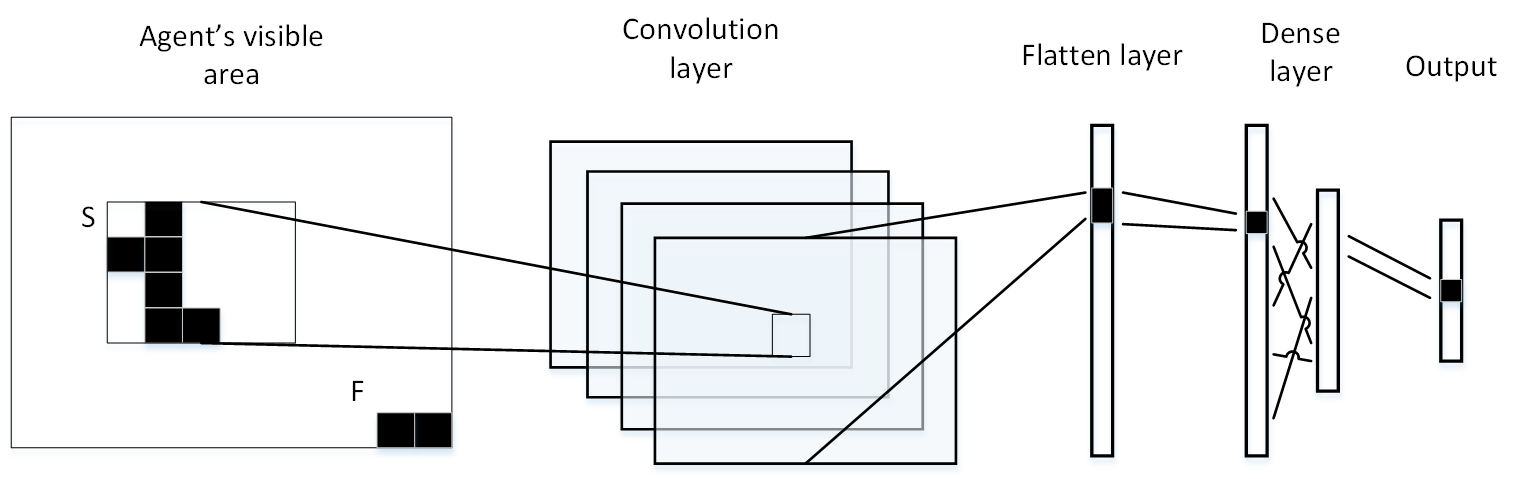
\includegraphics[width=0.8\textwidth]{examples/path/neural_arch.png}
	\end{frame}
	
	\begin{frame}
		\frametitle{Модели обучения в мозге}
		
		\begin{center}
			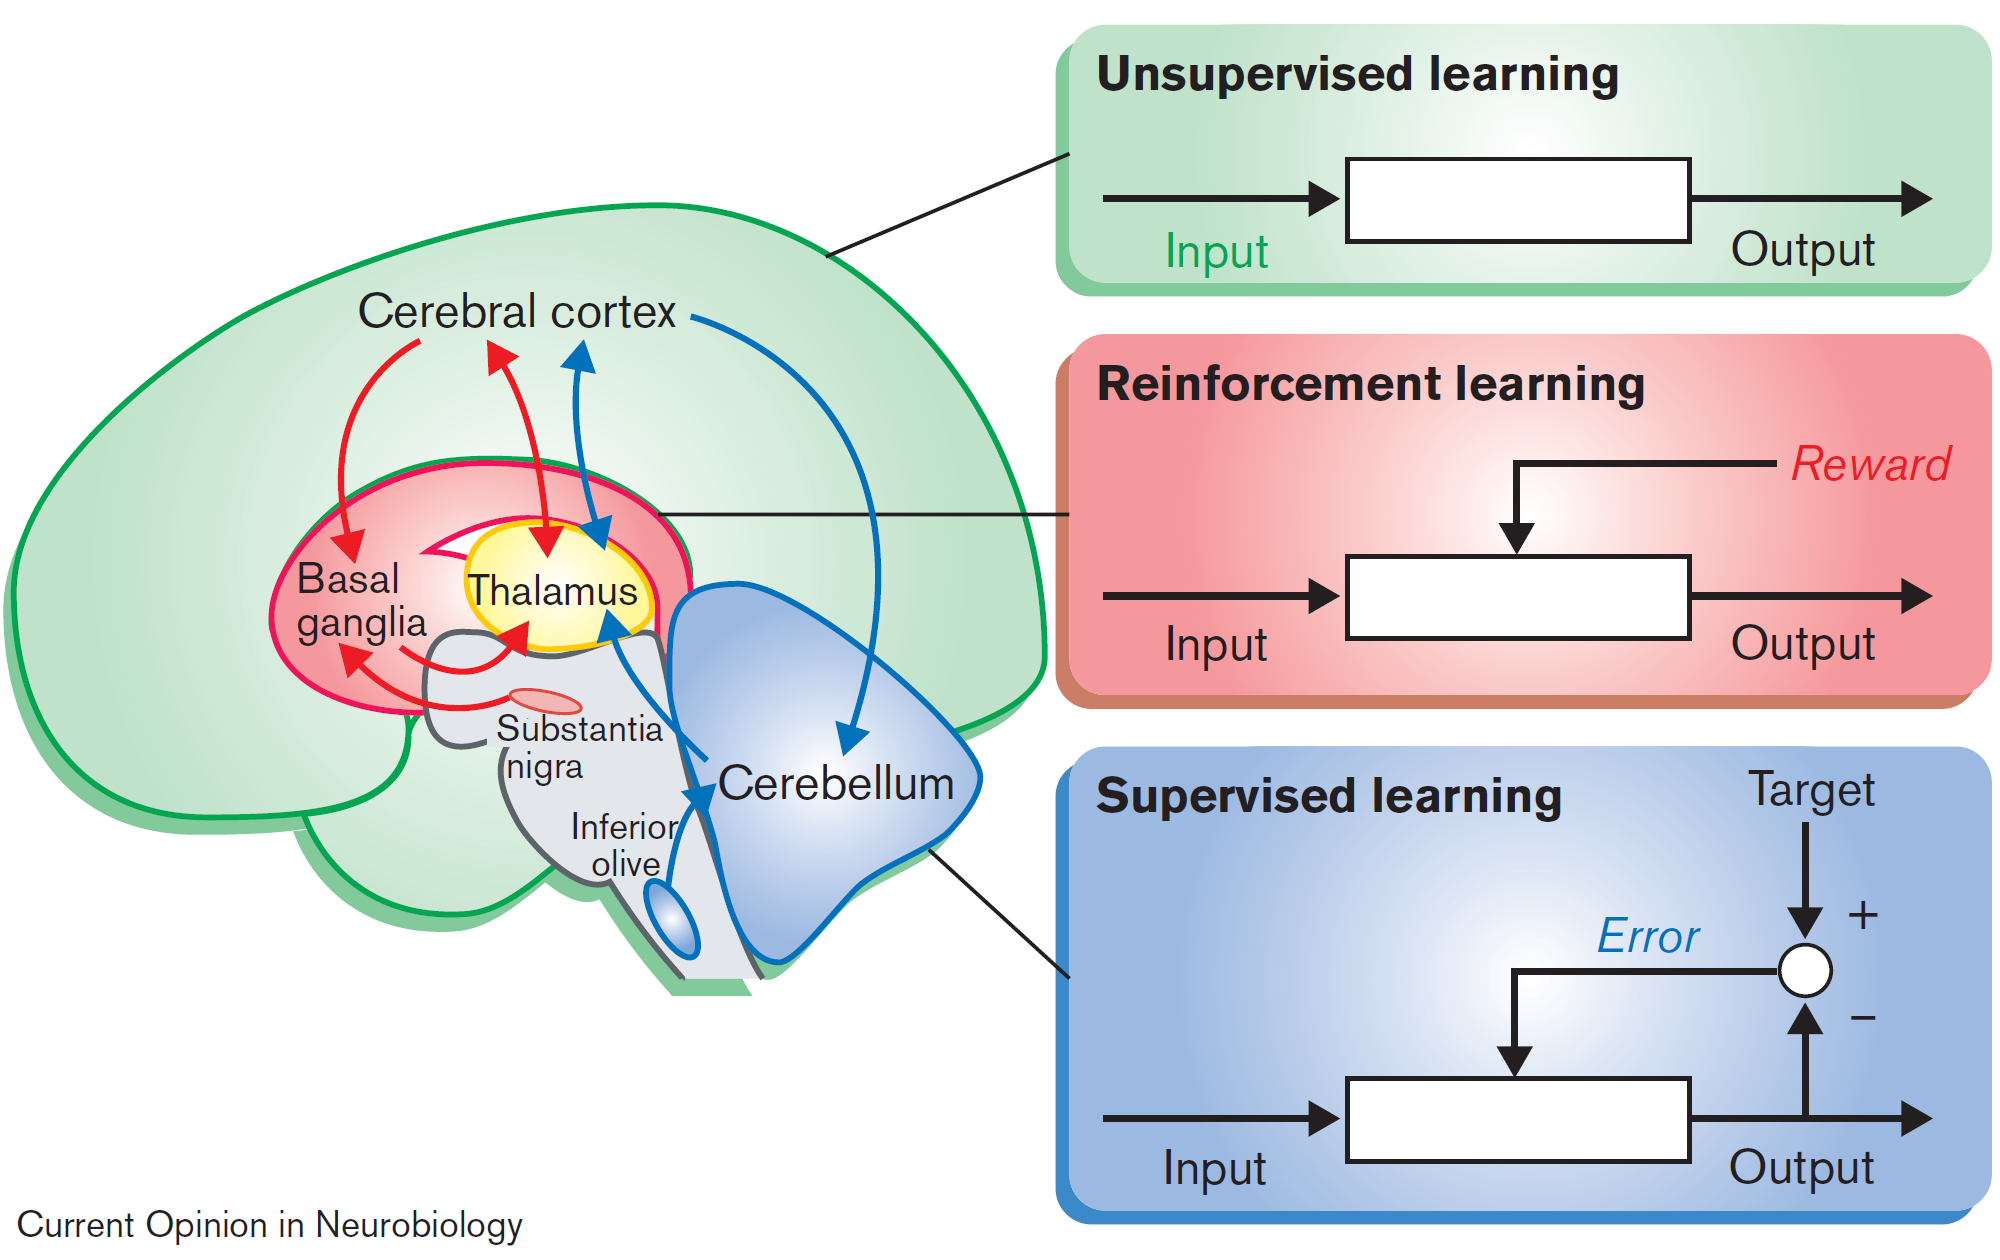
\includegraphics[width=0.8\textwidth]{misc/phisio/doya_schema}
		\end{center}

	\end{frame}	
	
	\begin{frame}
		\frametitle{Нейронный субстрат}
		
		\begin{columns}
		\begin{column}{0.35\textwidth}
			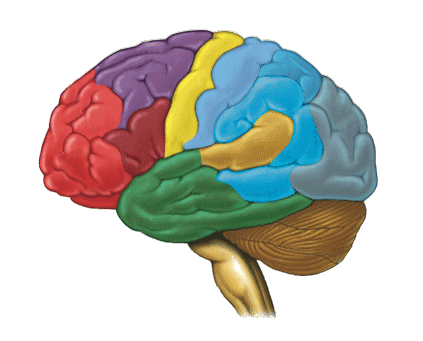
\includegraphics[width=0.8\textwidth]{misc/phisio/mozg_2}
			\par\bigskip
			\hspace{-7mm}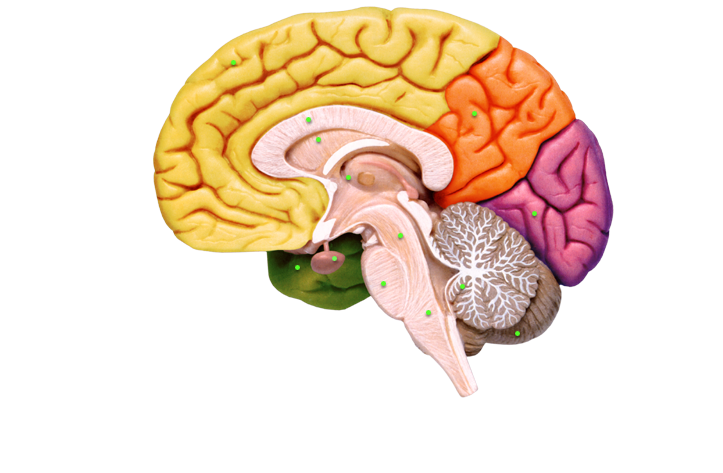
\includegraphics[width=\textwidth]{misc/phisio/mozg}
		\end{column}
		\begin{column}{0.65\textwidth}
			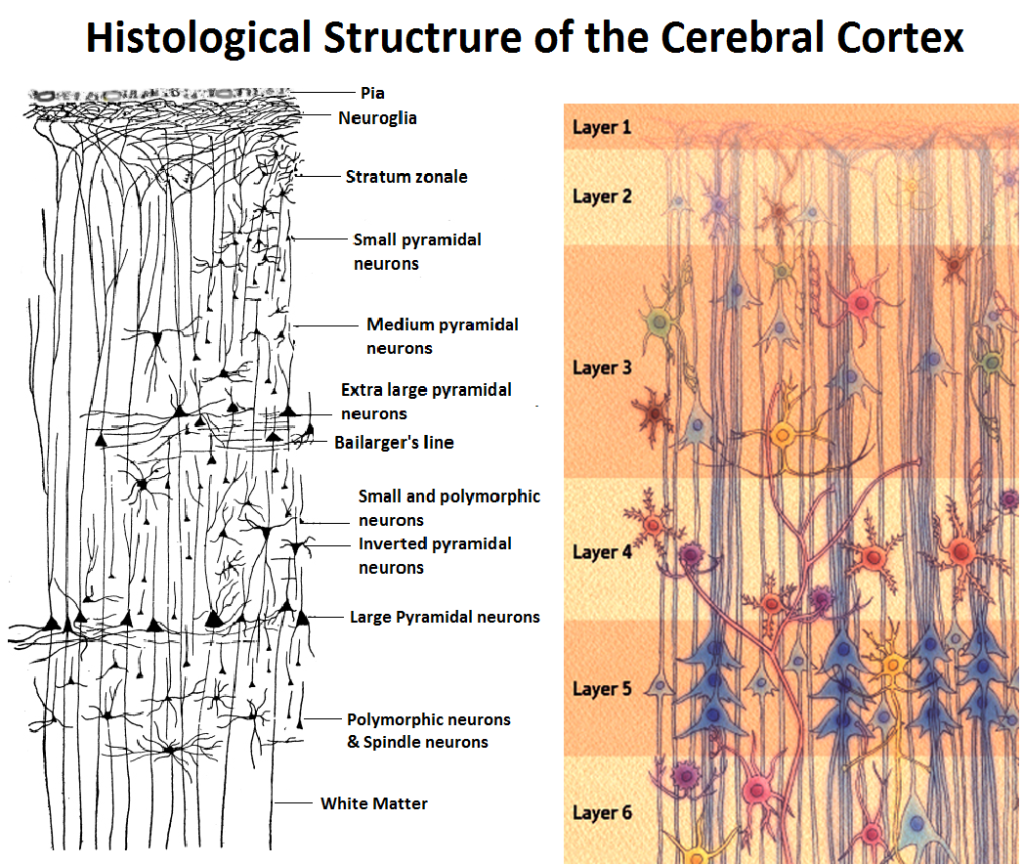
\includegraphics[width=\textwidth]{misc/phisio/cortex_layers}
		\end{column}
		\end{columns}

	\end{frame}
		
		
	\begin{frame}
		\frametitle{Иерархическая временная память}
		
		\begin{center}
		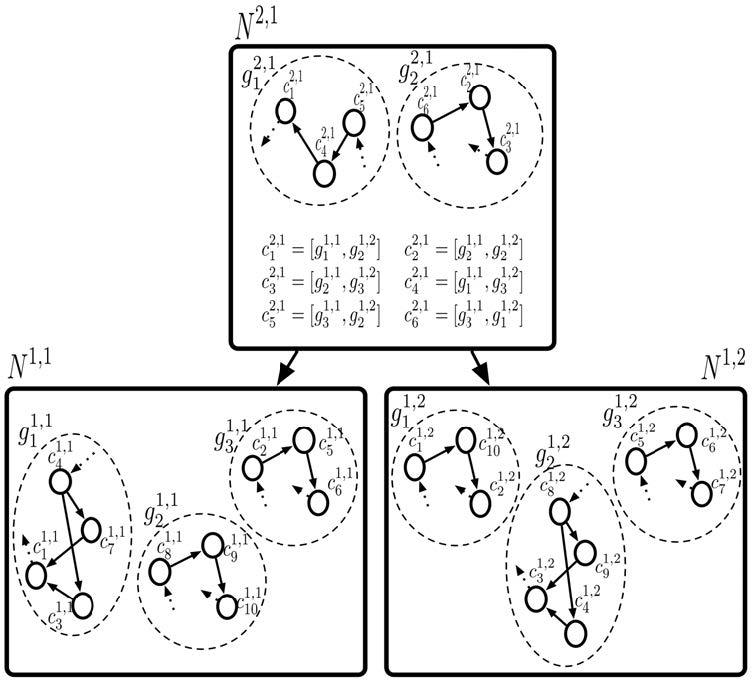
\includegraphics[width=0.5\textwidth]{misc/mpf/hawkins_htm}
		\end{center}
		\par\bigskip
		\begin{itemize}
			\item $N^{i,j}$ - узлы сети,
			\item $g^{i,j}$ - временные группы,
			\item $c^{i,j}_k$ - паттерн (синхронные шаблоны).
		\end{itemize}
				
	\end{frame}
		
	\begin{frame}
		\frametitle{Иерархическая временная память}
		
		\begin{center}
		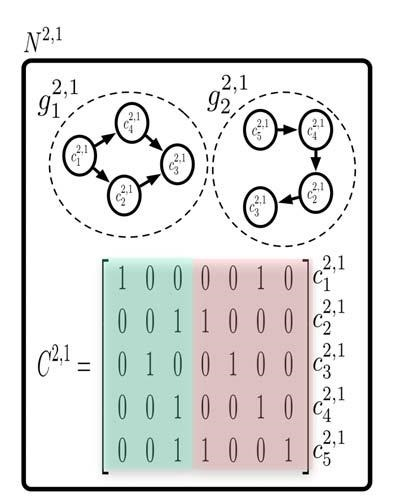
\includegraphics[width=0.3\textwidth]{misc/mpf/hawkins_htm_ex_a}
		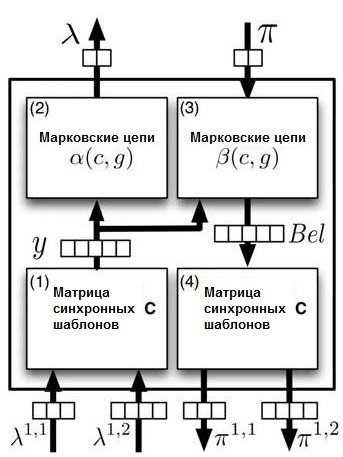
\includegraphics[width=0.3\textwidth]{misc/mpf/hawkins_htm_ex_b}
		\end{center}

	\end{frame}
	
	\begin{frame}
		\frametitle{ИВП: пример}
		
		\begin{center}
			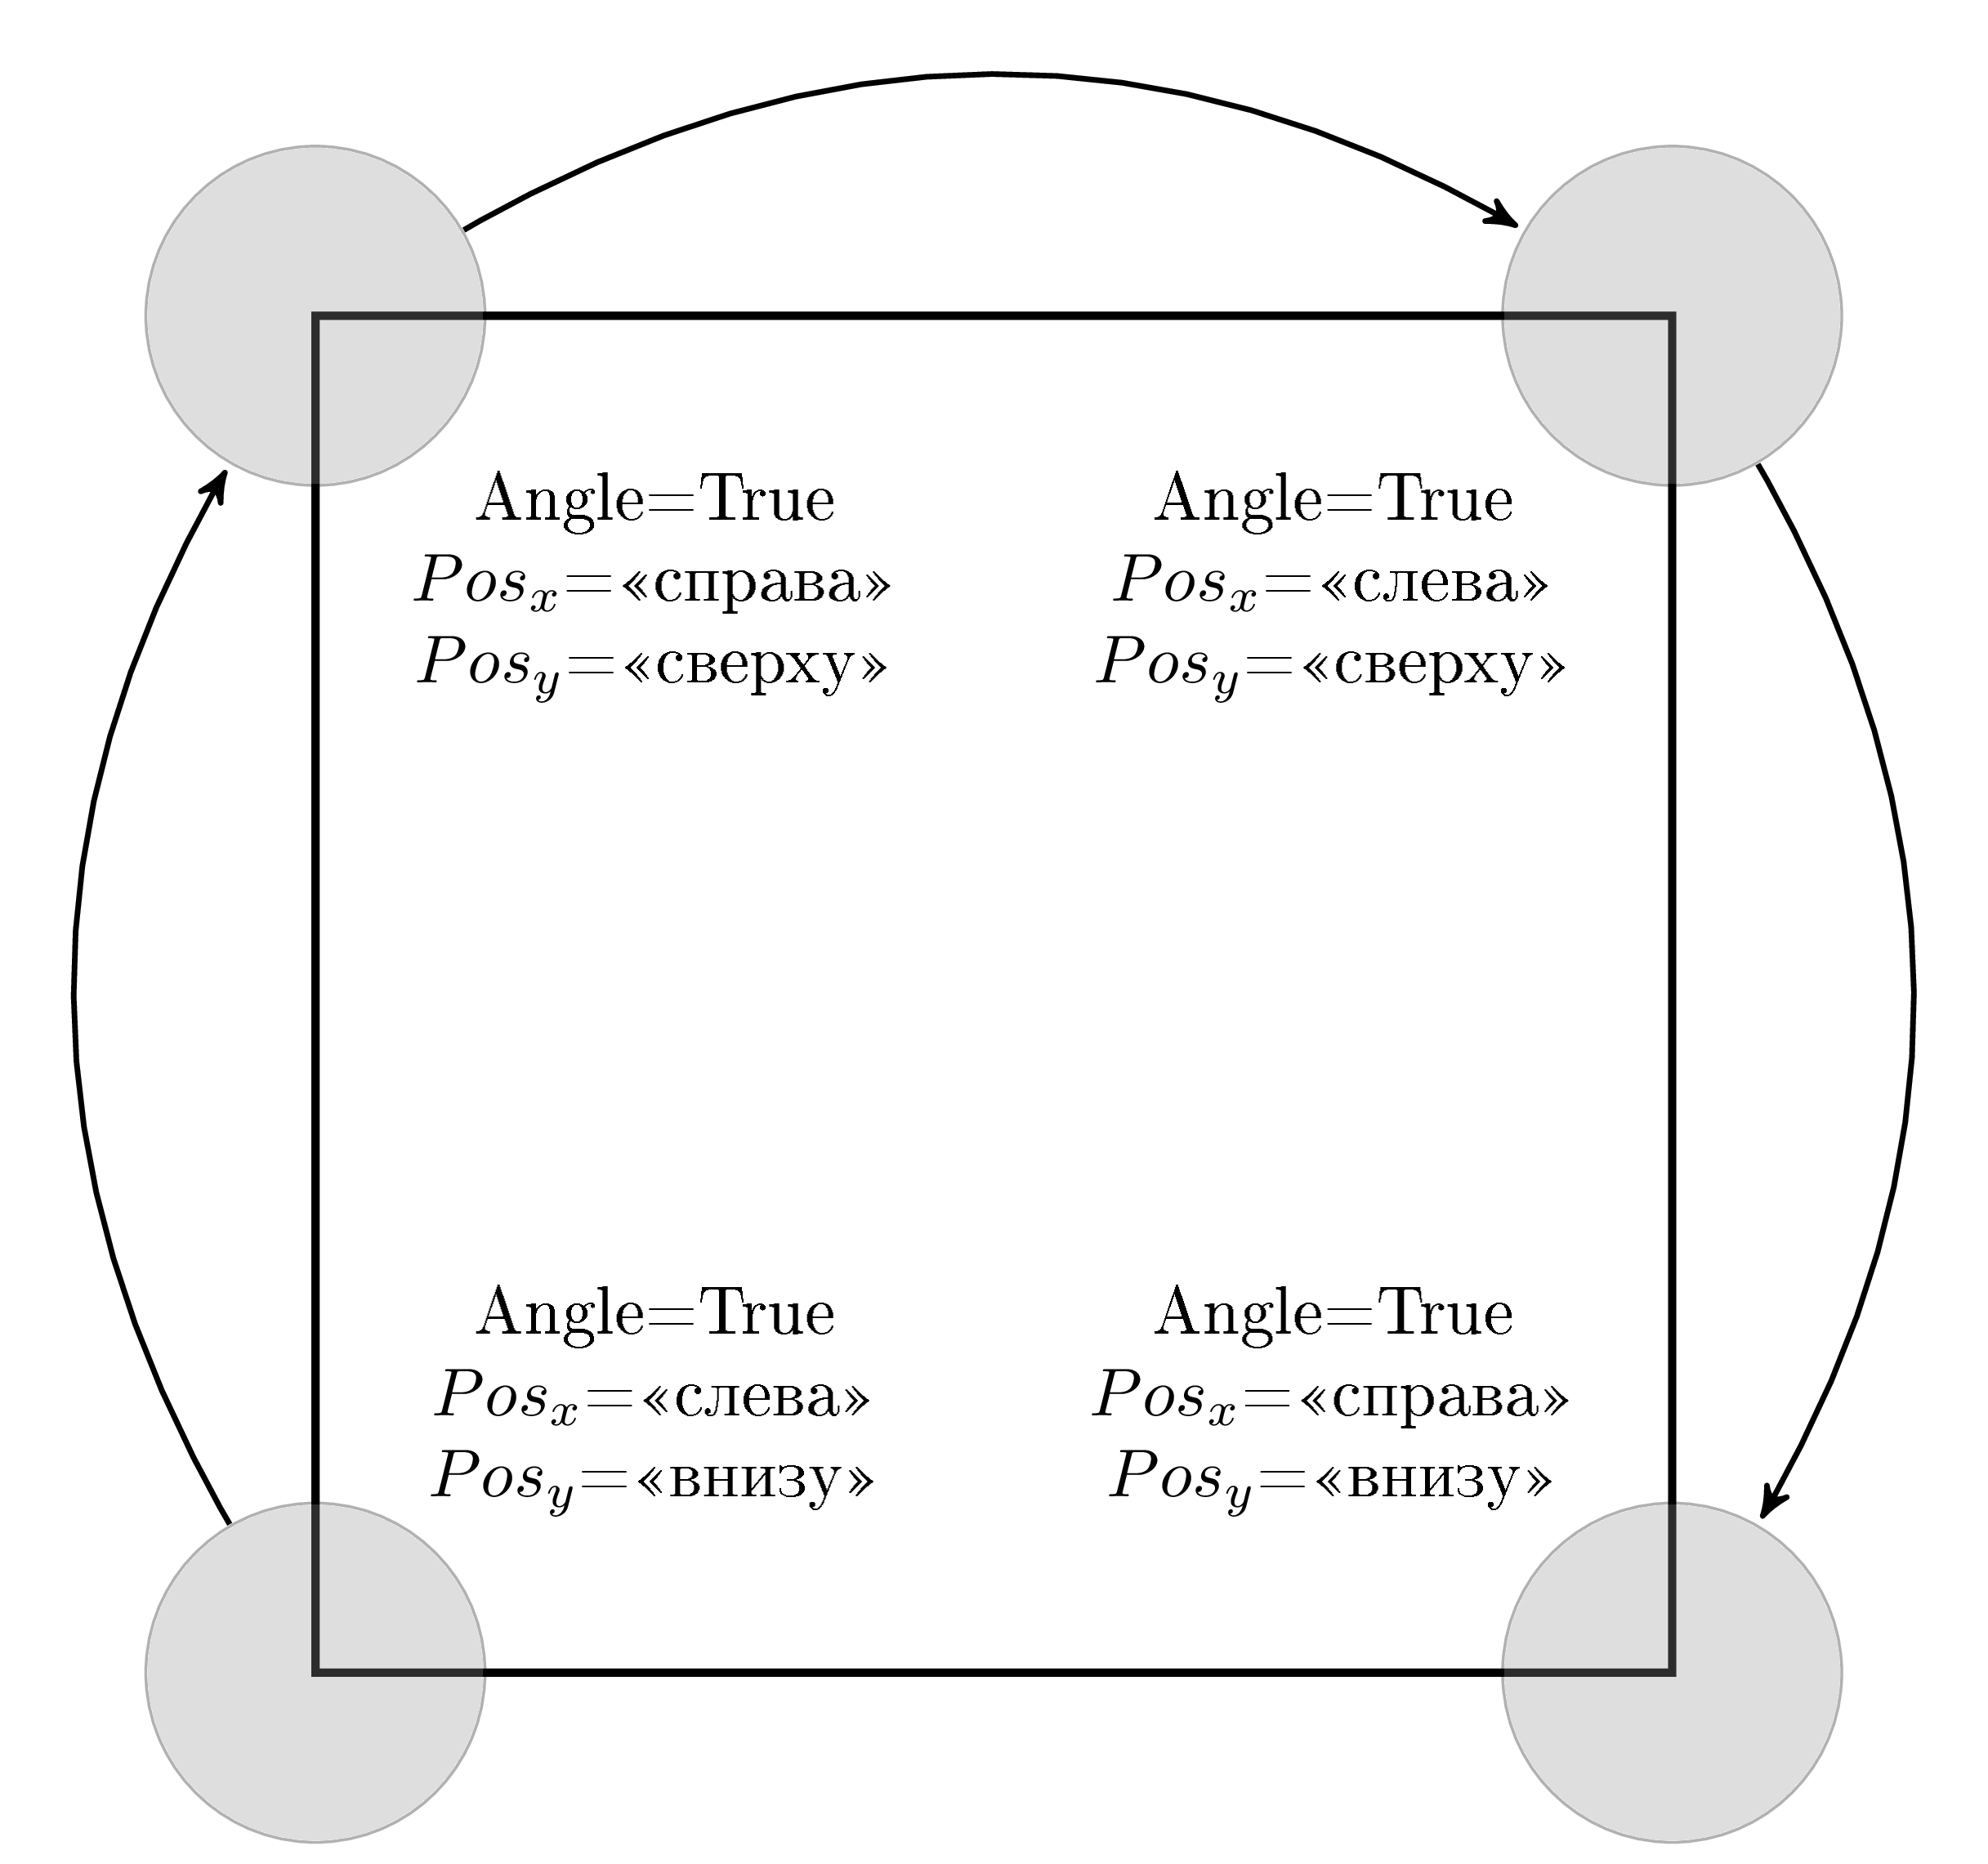
\includegraphics[width=0.4\textwidth]{examples/recognition/square.png}
			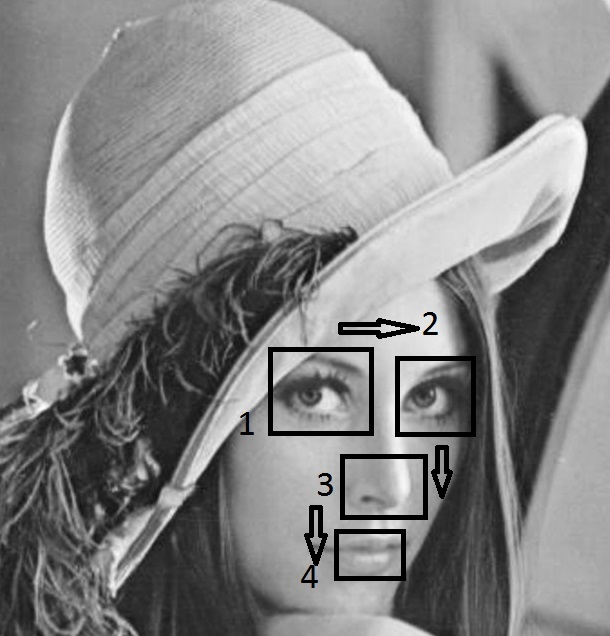
\includegraphics[width=0.4\textwidth]{misc/photos/face.jpg}
		\end{center}
		\begin{align*}
		z=\left[\begin{array}{cccc}
		1 & 0 & 0 & 0 \\ 
		0 & 1 & 0 & 0\\ 
		0 & 0 & 1  & 0\\
		0 & 0 & 0  & 1\\
		\end{array}\right]
		\end{align*}
	\end{frame}

	\begin{frame}
		\frametitle{Модель процесса обучения}
		
		К основным принципам работы механизма обучения относятся: 
		
		\begin{itemize}
			\item использование иерархии вычислительных узлов с восходящими и нисходящими связями, 
			\item использование Хэббовских правил обучения, 
			\item разделение пространственного и временного группировщиков, 
			\item подавление второстепенной активации для формирования разреженного представления.
		\end{itemize}
		
	\end{frame}	
	
	\begin{frame}
		\frametitle{Нейронная организация}
		
		\begin{columns}
		\begin{column}{0.65\textwidth}
		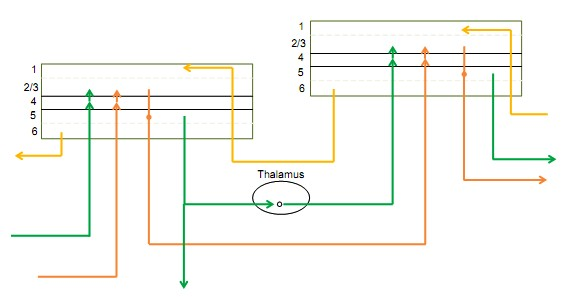
\includegraphics[width=0.9\textwidth]{misc/mpf/regions_connect}
		\end{column}
		\begin{column}{0.35\textwidth}
		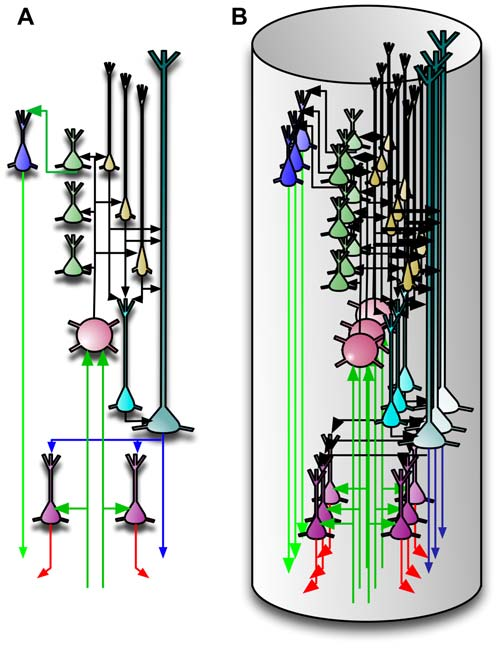
\includegraphics[width=\textwidth]{misc/phisio/column}
		\end{column}
		\end{columns}

	\end{frame}
		

\end{document}
	
	
